% Status: Zweitkorrektur
\subsection{Integration der Designvorlagen}
\label{Kommandozeilenprogramme}
Das Kommandozeilenprogramm zur Konvertierung der Adobe Illustrator-Dateien, welches in Abschnitt \ref{sect:Designvorlagen} beschrieben wird, als \emph{draftImporterCli} bezeichnet und dessen Abhängigkeiten werden durch Abbildung \ref{fig:DesignImport} dargestellt.
Die gestrichelten Pfeile stellen die Nutzung von Schnittstellendefinitionen dar und die durchgängigen Pfeile funktionale Abhängigkeiten. Es wird durch \lstinline|draftImporterCli.ts| auf den Ordner \lstinline|stores| zugegriffen. Da das Kommandozeilenprogramm Redux nicht nutzt, ist dieser Zugriff ungünstig.


\begin{figure}[H]
    \centering
    \caption{Abhängigkeiten des Kommandozeilenprogramms \emph{draftImporterCli}}.
    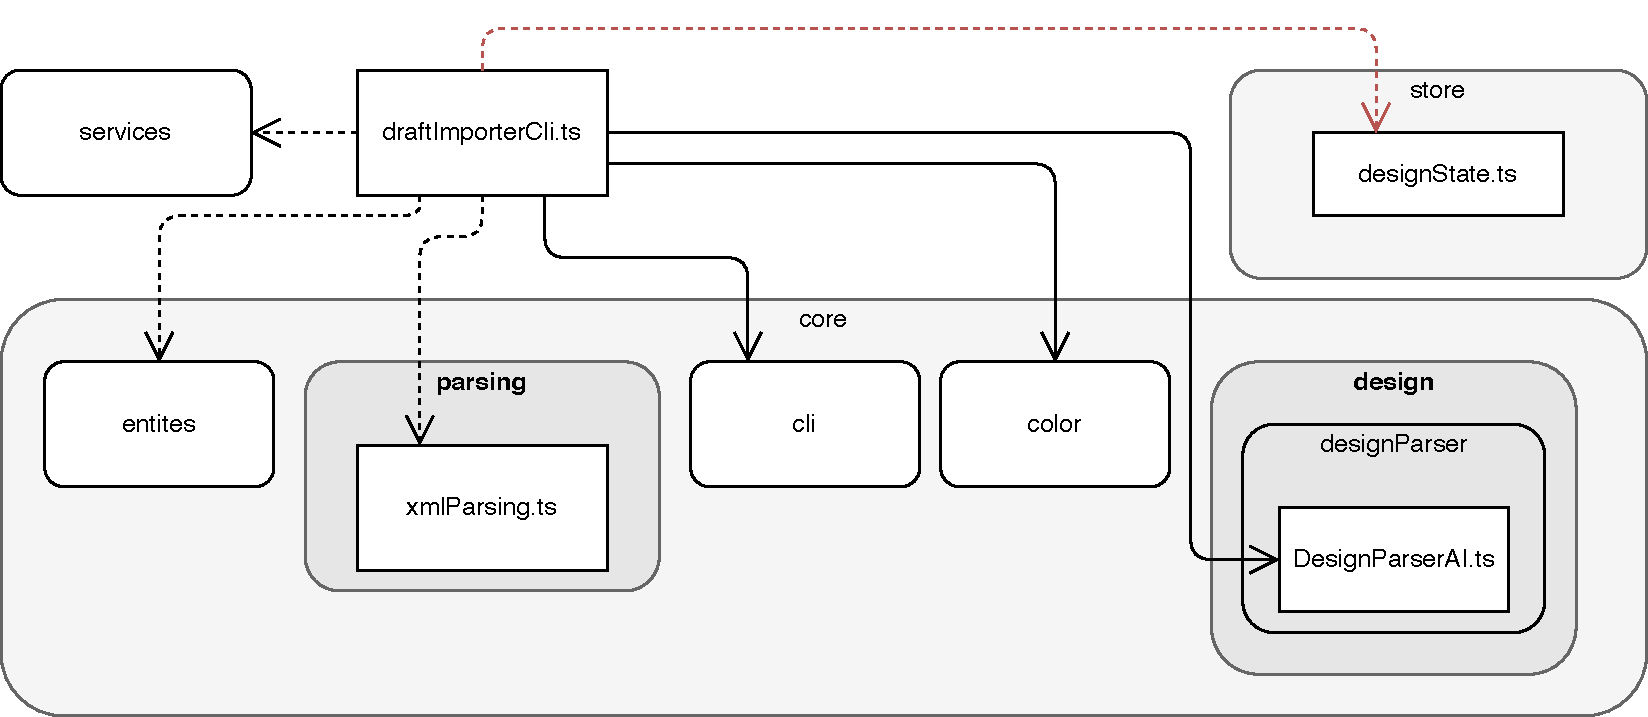
\includegraphics[width=.9\textwidth]{diagrams/Ist-Architektur/draftImporter-analysis.pdf}
    \label{fig:DesignImport}
\end{figure}
Ebenfalls in Abschnitt \ref{sect:Designvorlagen} wurde das Kommandozeilenprogramm zur Konvertierung der Designderivate zu SVG-Dateien beschrieben, welches als  \emph{designToSvgCLI} bezeichnet wird.
Das Programm liest ein Designderivat ein, welches dem Programm als Argument übergeben wurde. Das Programm konvertiert die einzelnen Designseiten in das SVG-Format und speichert sie als SVG-Dateien in einem Zielordner, welches ebenfalls dem Programm als Argument übergeben wird. 
Die Abhängigkeiten des Kommandozeilenprogramm werden durch Abbildung \ref{fig:DesignToSvg} dargestellt.

\begin{figure}[H]
    \centering
    \caption{Abhängigkeiten des Kommandozeilenprogramms \emph{designToSvgCLI}}.
    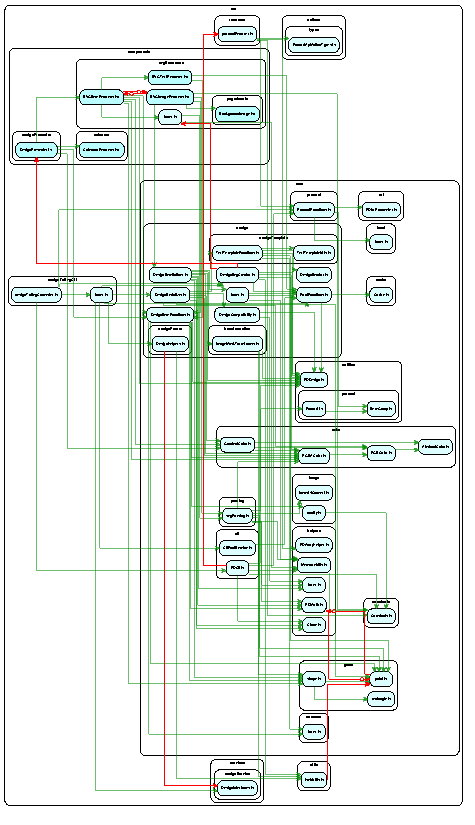
\includegraphics[width=.9\textwidth]{diagrams/Ist-Architektur/designToSvgCLI-analysis.pdf}
    \label{fig:DesignToSvg}
\end{figure}

